
\section{Material and methods}

\subsection{Simulation setup}

The monitoring system modeled in this simulation work is a Compton camera prototype under development within the French collaboration CLaRyS. The detectors detailed characteristics can be found in \cite{krimmer:hal-01101334}.\\
%Like most of the Compton camera devices, the CLaRyS prototype includes a scatterer and an absorber. 
The scatterer consists of seven parallel planes of silicon detectors (double-sided silicon strip detectors, DSSDs), $9\times9\times0.2$~cm$^3$, with 1~cm distance between the centers of two neighboring planes, while the absorber is composed of an array of $10\times10$ BGO (Bismuth Germanate - Bi$_{12}$GeO$_{20}$) blocks ($3.5\times3.5\times3.0$~cm$^3$ each) placed behind the silicon layers at a distance which can be tuned according to the requirements.

\begin{figure}	
  \centering
  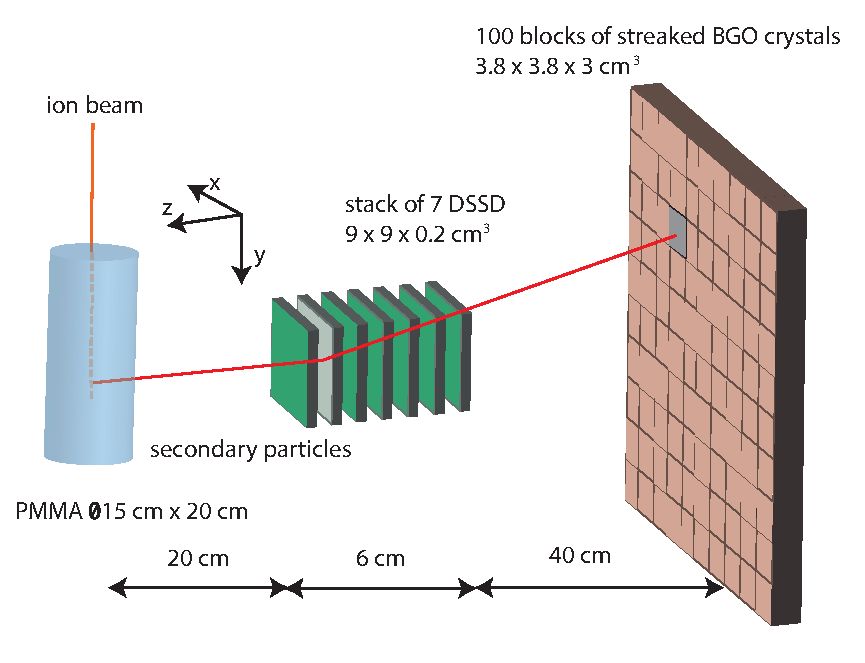
\includegraphics[width=0.7\textwidth]{./Figure/Compton_Camera_hadontherapy_PMMA_Cylinder_EN.pdf}
  \caption{Scheme of the simulation setup (not at scale): a PMMA cylindrical phantom is set in front of the Compton camera prototype. The Compton camera is composed of a stack of 7 double sided silicon strip detectors (scatterer) and a plan of 100 single BGO blocks. The set distances are realistic for clinical conditions. This geometrical configuration has been used for all the simulations presented in this work.}
  \label{fig:fig_setup_CC_simulation_Hadronth}
\end{figure}

The silicon detectors have a strip pitch of 1.4~mm, for a total of 64 strips per side (double-sided readout based on electron and hole pairs collection). 
Regarding the BGO blocks, their entrance surface is streaked in a 8$\times$8 matrix of pseudo-pixels, $4.4\times4.4$~mm$^{2}$ size, and the readout is performed via 4 photo-multiplier tubes. The position reconstruction is achieved via Anger logic.

A scheme of the simulation setup is given in figure~\ref{fig:fig_setup_CC_simulation_Hadronth}. The ion beam interacts with a cylindrical PMMA (PolyMethylMethAcrylate) phantom (15~cm diameter and 20~cm length) placed in front of the Compton camera as target. It is placed 20~cm far from the first silicon plane (center-to-center distance) which seems a realistic distance in clinical conditions. The distance between the last silicon layer and the absorber array (center-to-center) is set to 40~cm in order to permit time-of-flight measurements (see section~\ref{MatMeth::TOF_Ecut}).

The silicon detector strips are not reproduced in the simulation code, and the transverse spatial resolution is set to 0.9~mm FWHM at the reference energy of 1~MeV, according to preliminary measurements performed on smaller detector prototypes. Concerning the transverse direction (perpendicular to the beam line), the interaction position is set to the center of the involved silicon plane. A mono-block crystal is simulated for the absorber for simplicity. The events are selected to be limited to a single block component based on the interaction localization, and the interaction position is reconstructed via center of gravity calculation if multiple interactions occur. An uncertainty contribution, randomly extracted by a Gaussian of 5~mm FWHM, is added to the reconstructed position to mimic the pseudo-pixel-based readout. For what concerns the parallel direction, given the fact that the employed BGO blocks have not depth of interaction reconstruction capabilities, the interaction position is fixed to the center of the mono-block crystal.

The energy resolution of the BGO blocks was estimated in preliminary measurements and is accordingly set to 17\% FWHM at the reference energy of 667~keV (a 137-cesium source has been used for the measurements). The energy resolution of the silicon detector is set to 5~keV (FWHM) according to the design expectations.

The time resolution has been set to 3.0~ns FWHM for the BGO blocks and to 15.0~ns FWHM for the silicon slabs, according to preliminary measurements performed on test detector modules at the GANIL %(Grand Accelerateur National d'Ions Lourds) 
center in France.

The detector resolutions play an important role in the Compton camera performances. The spatial resolution of the absorber influences the position of the apex of the Compton cone as well as its axis orientation. The energy resolution of the scatterer determines the Compton cone aperture angle. The time resolution impacts the coincidence window between the absorber and the scatterer, and therefore the detectors ability to distinguish between true and random coincidences.

The CLaRyS project also includes the development of a beam tagging hodoscope, composed of scintillating fibers read out by multi-channel photomultipliers. This detector is used to synchronize the beam time and space structure to the prompt gamma detection in order to tune the detection window reducing the background contamination. In addition to this, the spatial localization of the impinging beam bunch can be included in the event reconstruction algorithm to add constraints to the obtained solutions (see section~\ref{MatMeth:reconstruction}). The hodoscope is not included in the simulation, but its spatial and time resolution have to be taken into account for the time-of-flight discrimination (see section~\ref{MatMeth::TOF_Ecut}) and events reconstruction. They are set to 1~ns and 1~mm FWHM, respectively.\\ 
The detector's spatial, energy, and time resolutions are summarized in table \ref{table:table_resolution_detecteurs_CC_simulation_Hadronth}.

\begin{table}
\centering
%\begin{tabular}{>{\columncolor[gray]{0.9}}ccc}
\caption{Estimations of reachable resolutions with the detectors. Those resolutions are applied during the simulations.}
\begin{tabular}{cccc}
\hline
\textbf{Resolution (FWHM) at 1~MeV} & \textbf{Scatterer} & \textbf{Absorber} & \textbf{Hodoscope}\\
\hline 
\textbf{spatial [mm]	}			 &     0.9		 &  5 &	 1\\
%\hline
\textbf{energy}				&	5~keV		&  17~\%	&	/\\
%\hline
\textbf{timing [ns]}	        		&	15			&	3 	&  1\\
\hline
\end{tabular}
\label{table:table_resolution_detecteurs_CC_simulation_Hadronth}
\end{table}
    
The Monte Carlo simulation is performed with the Geant4 toolkit, version 9.6.02. 
%Geant4 has been developed at CERN %(Conseil europ\'{e}en pour la recherche nucl\'{e}aire) for high energy physics experiments, but it has been shown that it can be used for ion beam therapy studies \cite{cirrone_hadrontherapy_2011,toshito_new_2010}. 
%Some improvements are still needed in order to extend the hadronic models to low energy applications~\cite{dedes_assessment_2014, Pinto:2016aa}.
The particle interactions in matter are described in this work by means of the models listed in table~\ref{table:table_modele_physic_CC_simulation_Hadronth}. Additionally, the Doppler broadening and the photon polarization effects are included.
 

\definecolor{Gray}{gray}{0.9}

\begin{table}
\label{physlist_ion}
\caption{Hadronic models used in the Geant4 simulations.}
\begin{scriptsize}
\begin{center}
\renewcommand{\arraystretch}{1.2}
%\begin{tabular} {>{\columncolor[gray]{0.9}}cccc}\hline  
\begin{tabular} {cccc}\hline
%\rowcolor{Gray}
\textbf{Process} & \textbf{Protons} & \textbf{Ions} & \textbf{Neutrons} \\ \hline 
\textbf{Electromagnetic} & \multicolumn{3}{c}{standard$_{\rm{option3}}$} \\ %\hline
\textbf{Inelastic} & G4BinaryCascade & G4QMDReaction  &  G4BinaryCascade  \\ 
 & & (G4IonsShenCrossSection)&+ G4NeutronHPInelastic ($<$19~MeV)\\ %\hline
\textbf{Elastic} & G4LElastic & G4LElastic & G4LElastic + G4NeutronHPElastic ($<$19~MeV)\\ %\hline
\textbf{Fission} & / & / & G4LFission + G4NeutronHPFission($<$19~MeV) \\ %\hline
\textbf{Capture} & / & / & G4LCapture +  G4NeutronHPCapture ($<$19~MeV) \\ %\hline
\textbf{Radioactivedecay} & / & G4Radioactivedecay & / \\ \hline
\end{tabular}
\end{center}
\end{scriptsize}
\label{table:table_modele_physic_CC_simulation_Hadronth}
\end{table}

%\subsection{Data processing}
%\label{subsection:Treatment_data_CC_hadrontherapy_Geant4}

\subsection{Beam structure}
\label{subsection:modelisation_fasceau_ions_CC_hadrontherapy_Geant4}
\subsubsection{Beam structure measurements at HIT}
Our group performed a set of measurement to characterize the time structure of the synchrotron installed in the Heidelberg Ion Therapy Center (HIT), Germany~\cite{HIT_timeStructure}.
This beam structure is extrapolated from measurements performed by our group in 2013 at HIT; the beam time structure was measured for 200~MeV/u and 400~MeV/u primary ion energy with a two-fiber hodoscope (basic prototype of the one at present under development) and the spill signal was given by the accelerator. Figure \ref{fig:fig_structure_temps_faisceau_HIT_2013_CC_simulation_Hadronth} shows the beam structure for carbon ions at 400~MeV/u. The pulses have a spill period of 150.2~ns and each bunch is approximately 21.5~ns.
The mentioned measurements have shown that the spill phase changes during the extraction: this implies that the HF signal from the synchrotron can not be used to trigger the pulses, so that the use of an additional beam time stamp system like the hodoscope seems required for time-of-flight background rejection purposes.

\begin{figure} [!hbtp]	
  \centering
  %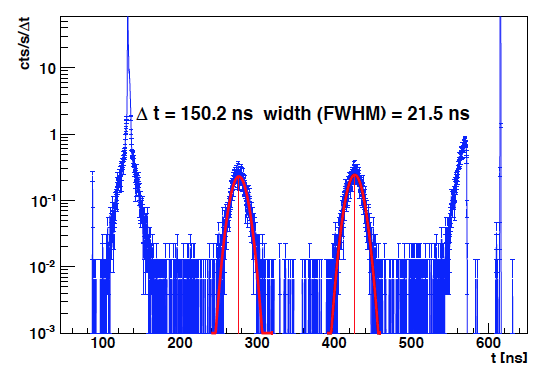
\includegraphics[width=0.6\textwidth]{./Figure/2013_Structure_Time_Beam_400MeV.png}
  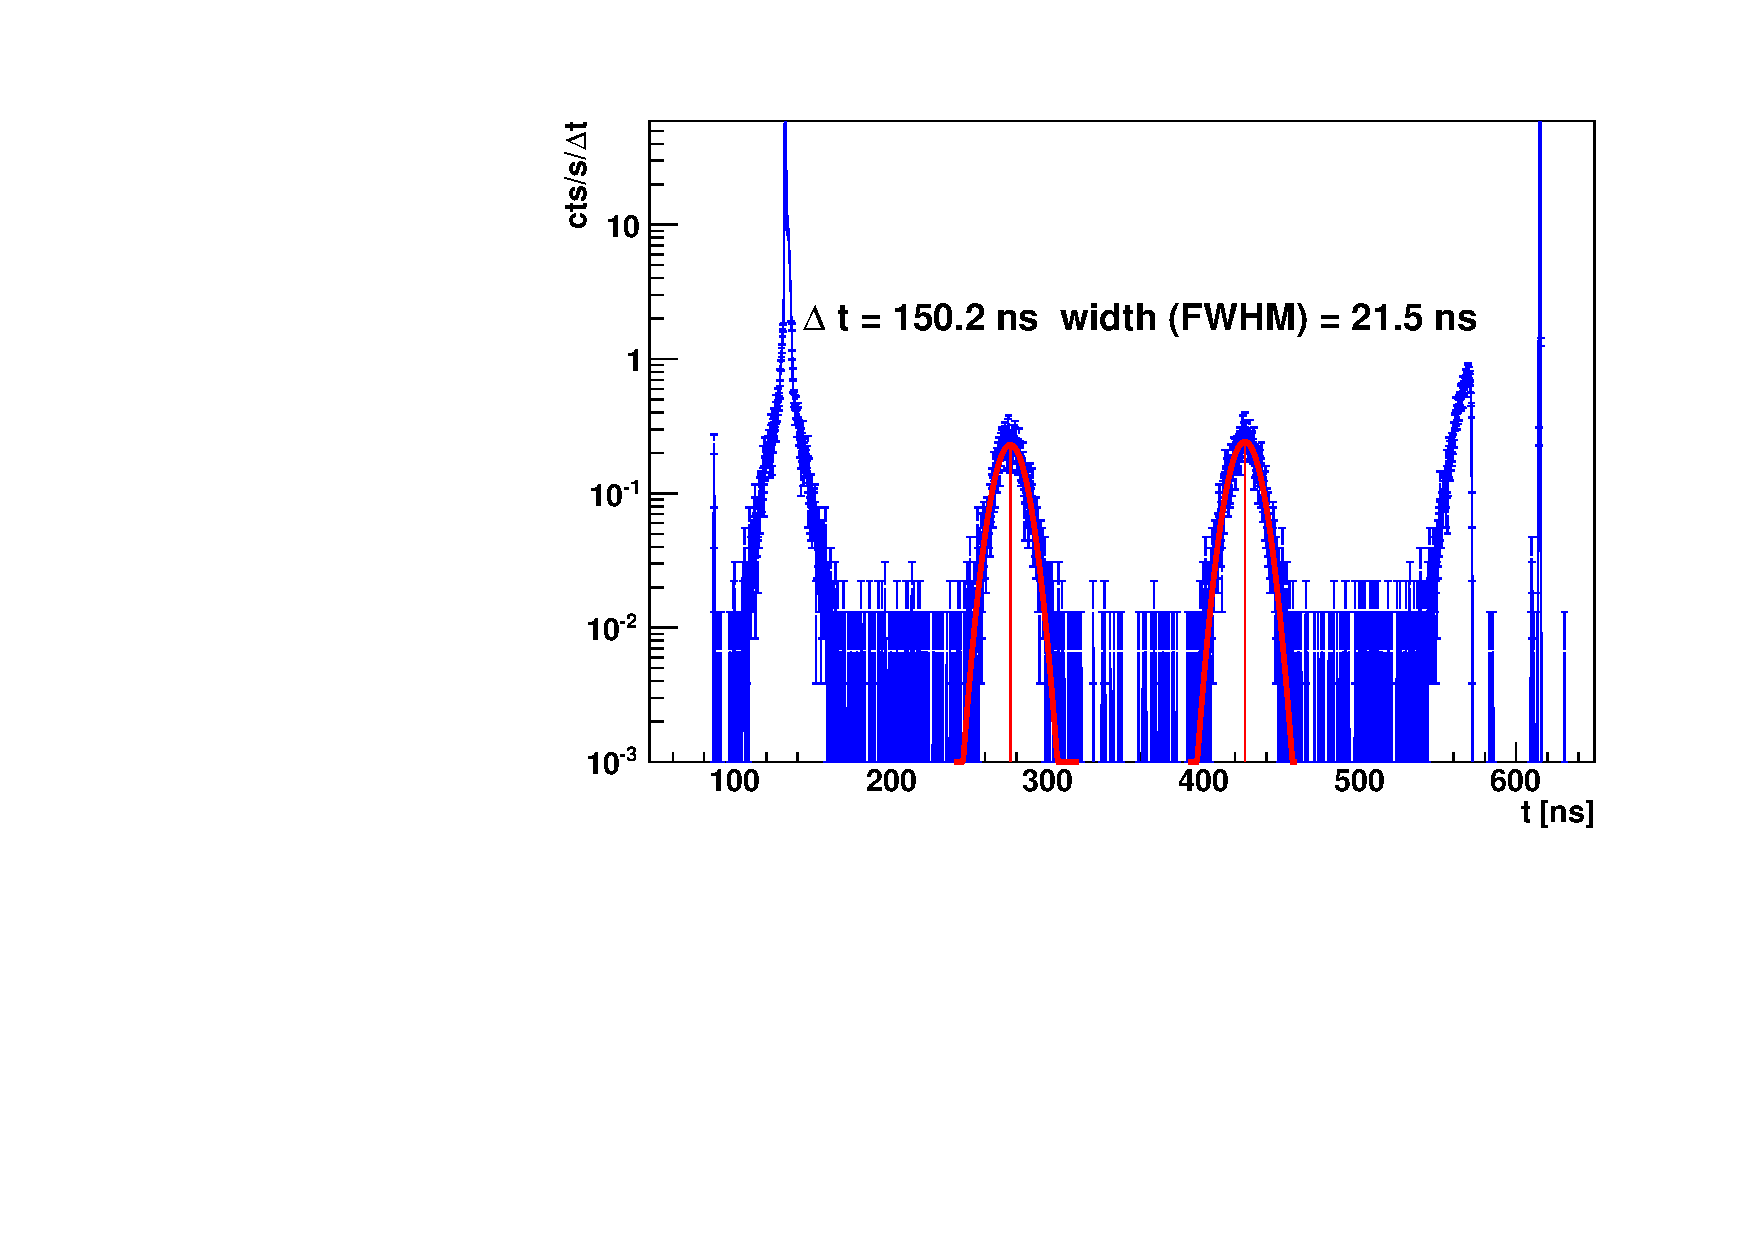
\includegraphics[width=0.6\textwidth]{./Figure/fiber_vert_hor_run14.pdf}
  \caption{Time micro-structure measured from a carbon ion beam at 400~MeV/u delivered at HIT. The pulses have an extraction period of 150.2~ns and the bunches are 21.5~ns FWHM. The measurement was achieved with a two-scintillating-fiber hodoscope. DA METTERE VERSIONE VETTORIALE}
  \label{fig:fig_structure_temps_faisceau_HIT_2013_CC_simulation_Hadronth}
\end{figure}


\subsubsection{Beam modeling}
The two main beam particles used in clinics are considered: protons and carbon ions. The beam range of interest is 15.2~cm in the PMMA phantom, and the associated energy is 160~MeV for protons and 305~MeV/u for carbon ions.\\ 
The beam transverse dimension is modeled with a Gaussian distribution with a standard deviation of 5~mm for protons at 160~MeV and 3.5~mm for carbon ions at 305~MeV/u. The number of incident ions for a spot in pencil beam scanning (PBS) mode is $10^8$ for protons (distal spot) and $10^5$ for carbon ions.\\
The beam time structure is applied at the data analysis stage.
Two different time structures have been considered for this study, related to two kinds of accelerators used in clinical practice: the IBA C230 cyclotron for protons (used in 16 clinical centers worldwide) and the HIT synchrotron for carbon ions. For protons at 160 MeV, the primary particles are grouped in bunches of 2~ns (this value may vary also according to the distance between the cyclotron and the treatment room, and energy spread selection) at a frequency of 106~MHz (9.42~ns)~\cite{Roellinghoff_2014}. The clinical beam intensity is 3.2~nA which corresponds to about 200 protons per bunch. Concerning the carbon ion beam at 305~MeV/u, the estimated microstructure during the extraction phase is composed of 30~ns duration bunches at a frequency of 5.9~MHz (170~ns period). The clinical beam intensity for carbon ions is $5\times10^7$~ions/s during extraction, corresponding to about 9~ions per bunch. 

The coincidence window (between scatterer and absorber events) is set to 40~ns, centered on each absorber detected interaction. This value is adapted to the detectors time resolutions. Table~\ref{table:definition_beam_structure_CC_hadrontherapy_Geant4} summarizes the presented beam time structures and coincidence reconstruction features.

\begin{table} [!htbp]
\footnotesize
\centering
\caption{Description of the two beam structures studied: the IBA cyclotron C230 for protons and the synchrotron installed at the Heidelberg Ion Therapy Center (HIT) in Germany for carbon ions. The macro-structure of the synchrotron, at the second time scale, is not considered here. The beam structures are applied to the simulation data.}
\setlength{\tabcolsep}{2pt}
%\hspace{-2.1cm}
\begin{tabular}{c|c|cc}
%\cline{2-4}
\hline
		\multicolumn{2}{c}{ }		 & 					\textbf{Protons} & \textbf{Carbon ions}\\ 
\hline
%\cline{2-4}%\hline
\multirow{3}{*}\textbf{Clinical features}		&	Facility	& IBA Cyclotron C230 &   Synchrotron at HIT\\
											& Clinical intensity& $  2\times10^{10}$ p/s  & $  5\times10^{7}$ ions/s\\
											& Energy 			&160~MeV 			&    305~MeV/u\\
%\cline{2-4}%
\hline
\multirow{3}{*}\textbf{Beam structure}		&	Bunch time [ns]	& 3.2				&  30\\
											& Period [ns]		&   9.4 				& 170\\
											& Primaries/bunch 	&217 			& 9\\
%\cline{2-4}%
\hline
\multirow{2}{*}\textbf{Detectors}						& Coincidence window [ns]		& 40 	&  40 \\
											&Time resolution (FWHM) [ns] & \multicolumn{2}{c}{Si: 15 and BGO: 3}\\
%\cline{2-4}%
\hline
\end{tabular}
\label{table:definition_beam_structure_CC_hadrontherapy_Geant4}
\end{table}



%\newpage
%---------------------------------------------------------------
%---------------------------------------------------------------
\subsection{TOF and energy based data selection}
\label{MatMeth::TOF_Ecut}

The Compton detection principle is based on a double interaction in the scatterer and absorber section, where an interaction is defined as an energy deposit in a detector module. As discussed in section~\ref{subsection:modelisation_fasceau_ions_CC_hadrontherapy_Geant4}, the coincidence reconstruction relies on a defined time window, fixed according to the detector resolution. In a simulation environment, different kinds of coincidence events can be distinguished and studied: 
\begin{itemize}
\item[-] real coincidences: created by a single photon first interacting in a single scatterer plane and then in a single absorber block;
\item[-] quasi-simultaneous interaction of two secondary particles;
\item[-] double interaction of the same particle, not a photon (protons, neutrons).
\end{itemize}

In an experiment the collected data are affected by a certain number of the so-called random coincidences, which cannot be experimentally distinguished from true coincidences, from the timing coincidence point of view. The amount of random coincidences depends on the detector time resolutions, on the fixed time coincidence window and on the beam time structure, on the phantom composition and camera prototype setup. In figure~\ref{fig:fig_explication_coincidence_CC_simulation_Hadronth}, a schematic view of the different kinds of coincidences is presented.

\begin{figure}
  \centering
  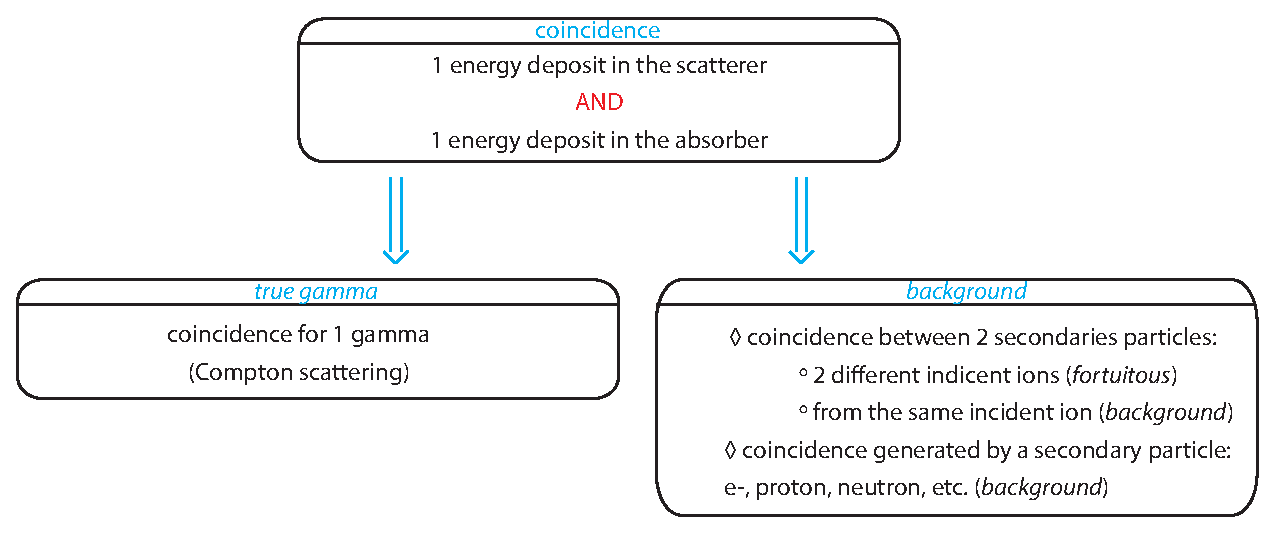
\includegraphics[width=0.9\textwidth]{./Figure/Schema_coincidence_EN.eps}
  \caption{Diagram showing the different definitions of coincidences in the Compton camera.}
  \label{fig:fig_explication_coincidence_CC_simulation_Hadronth}
\end{figure}

In addition to this, the prompt gamma measurement is contaminated by other secondary particles (mainly massive and charged particles like protons and neutrons), produced by the interaction of the primary particles with the patient/phantom.
Ad-hoc filtering methods are applied to reduce the above described contamination.

\begin{itemize}
\item Time-Of-Flight: it has been demonstrated by our group that a time-of-flight discrimination is possible and effective in reducing the background generated by massive particles interactions~\cite{Testa:2010aa}. The massive particles approach the detector at a lower speed with respect to photons. The time information provided by the hodoscope and the absorber can be combined to fix a detection time window and reject all the events outside the window. The time elapsed between the incident particle creation and the secondary particle detection in the absorber is considered as the time-of-flight. The hodoscope time resolution $u_{\mathrm{hodoscope}}$ (1~ns FWHM) is applied to the primary particle creation time, with a contribution randomly extracted from a Gaussian with $\sigma\,=$ 1/2.35~ns. The detection time in the absorber is affected by the absorber time resolution.

 \begin{eqnarray}
TOF = t_{\mathrm{absorber}}-t_{\mathrm{hodoscope}} \\
TOF_{\mathrm{simulation}} = t_{\mathrm{absorber}}-(t_{\mathrm{creation}} + u_{\mathrm{hodoscope}})
\label{TOF_equation}
\end{eqnarray} 

The time-of-flight spectrum resulting from the simulation shows that the coincidences of interest (produced by prompt-gamma rays) are included in a window between 0 and 8~ns (figure \ref{fig:fig_TOF_distribution_CC_simulation_Hadronth}). Therefore, all the coincidences with a TOF higher than 8~ns have been rejected.
\begin{figure}	
  \centering
  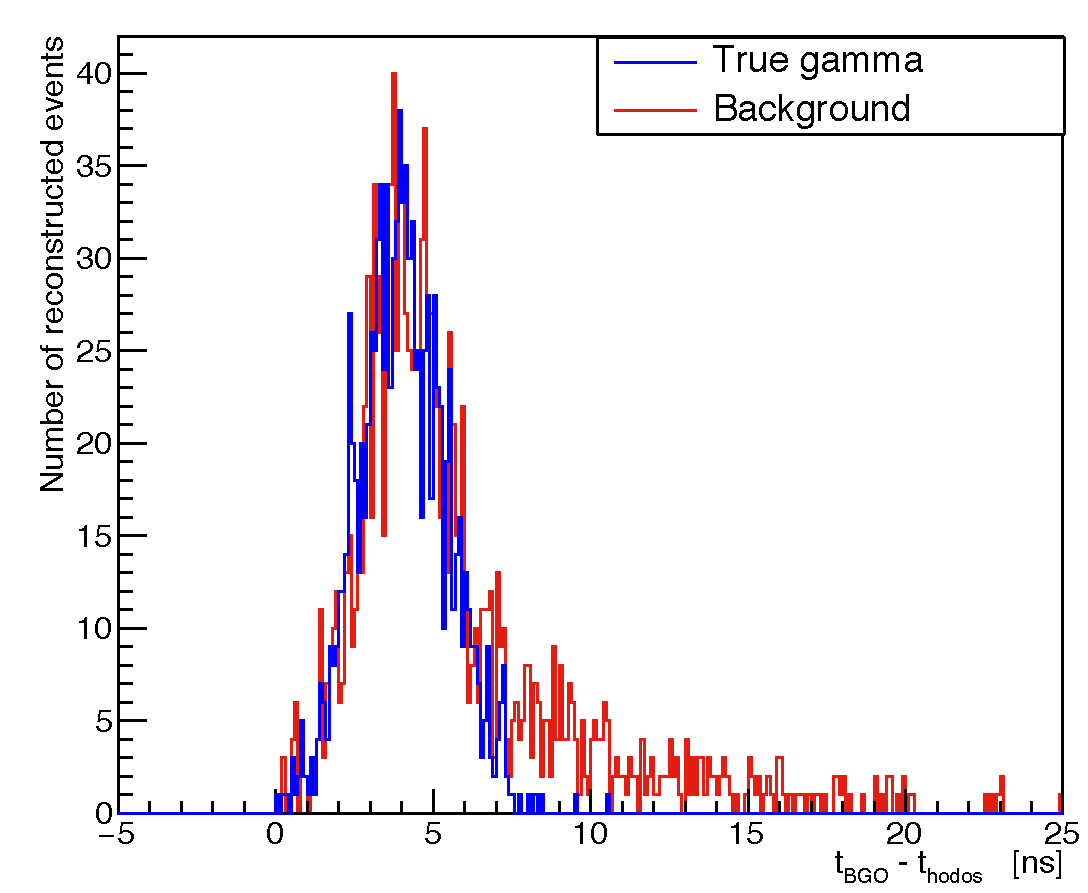
\includegraphics[width=0.6\textwidth]{./Figure/TOFspectra_2}
  \caption{Time of flight spectra of true gamma coincidences (blue) and background events (red) obtained with $10^{8}$ 160~MeV incident protons. The detection time for the absorber is given by the first deposit energy.}	
  \label{fig:fig_TOF_distribution_CC_simulation_Hadronth}
\end{figure}

\item Energy selection: energy thresholds are defined for the event detection. 50~keV and 100~keV are set as lower threshold for the energy deposited in a single silicon layer and absorber, respectively. For a complete event, a total absorbed energy lower limit is set to 1~MeV. In addition to the effect of background rejection, this selection also reduces the impact of partially absorbed photons and events with Compton electron escape.

Further energy selections, assuming for instance $E_1+E_2$ equal to one of the strong gamma lines, have been applied by other authors. Also, filters checking the possibility of reconstructing a Compton cone could be used. At this stage we did not consider such approaches, in order to cope with simple considerations on signal to noise on raw data.

\end{itemize}

\subsection{Reconstruction algorithms}
\label{MatMeth:reconstruction}
Once the coincidences are defined and selected according to the fixed physical cuts, the prompt-gamma emission point has to be reconstructed for each event. This can be done via analytic or iterative algorithms based on the Compton kinematics. Both are presented in the following sections.


\subsubsection{Line-cone algorithm}
The reconstruction via line-cone algorithm exploits the energy deposit and position information collected by the camera in addition to the beam planned path. Thanks to the deposited energies in the detectors and the interaction positions, a cone surface is analytically defined via the Compton equation~\ref{Compton_equation}. Figure~\ref{fig:reconstruction_scheme} shows a sketch of the reconstruction principle. The interaction position in the scatter gives the cone apex and the line connecting the interaction positions in scatterer and absorber gives the cone axis. We assume that the initial energy of the gamma ray is fully absorbed in the absorber. In order to constrain the reconstruction, the beam direction is used to limit the possible solutions (lying on the reconstructed cone surface) to two points (intersection of the beam direction and the reconstructed cone). The set of all the reconstructed points gives the emission source distribution. The final image is the mono-dimensional projection of the prompt gamma emission spectrum. 

\begin{figure}
\centering
  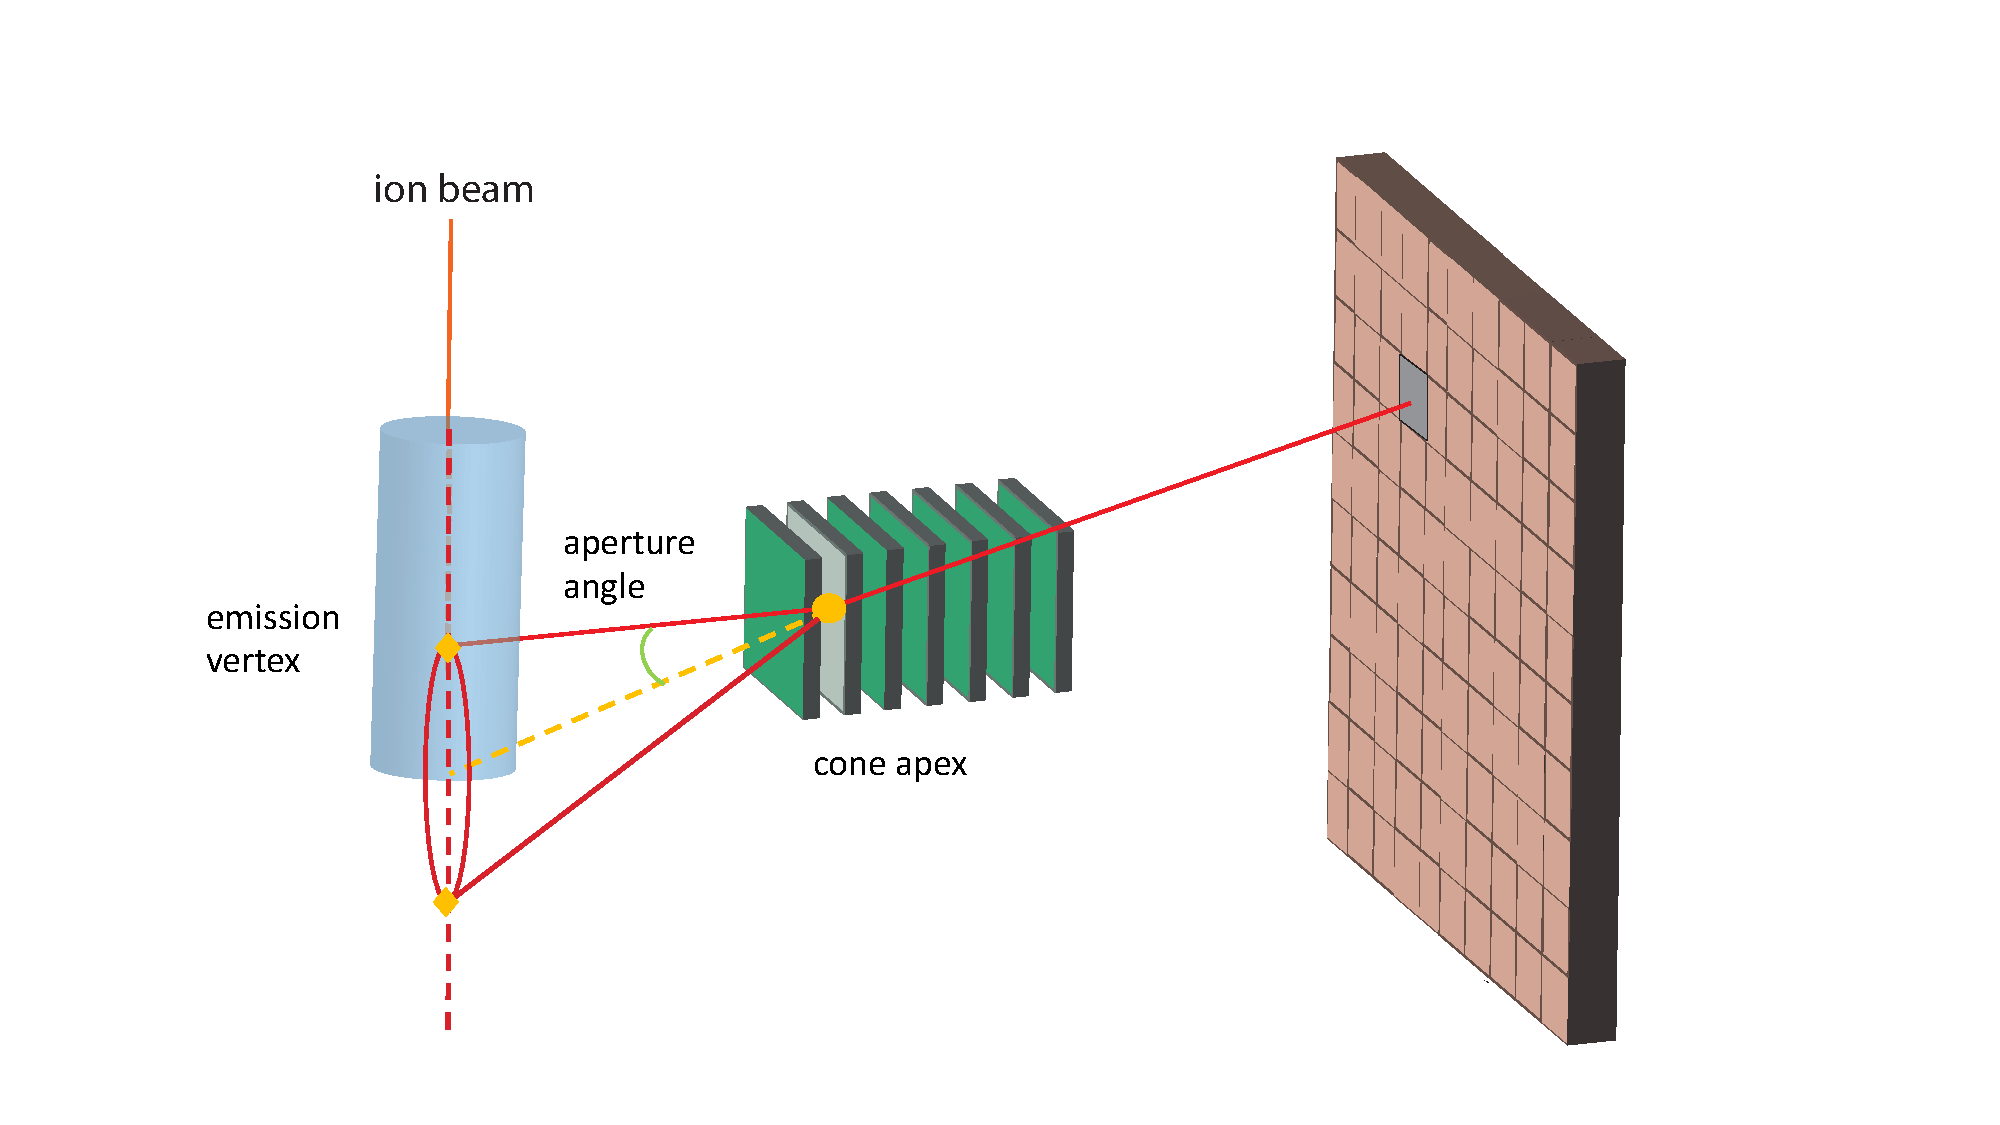
\includegraphics[width=0.8\textwidth]{./Figure/reconstruction_scheme}
  \caption{Scheme of the reconstruction principle for Compton events. For line-cone reconstruction methods, two points are extracted for each event (diamonds in the figure), provided by the intersection between the reconstructed Compton cone and the beam line. The reconstructed image is strictly 1D. For the iterative MLEM algorithm, each algorithm iteration adds constraints to the reconstructed cone surfaces, leading to  a 3D image.}	
  \label{fig:reconstruction_scheme}
\end{figure}

\subsubsection{LM-MLEM algorithm}	
The iterative methods allow to get a 3D image reconstruction, potentially by taking into account the spatial resolution and the energy resolution of the detectors. Few iterative algorithms have been developed for Compton event reconstruction~\cite{schone_common_2010, zoglauer_design_2011,gillam_compton_2011,mackin_evaluation_2012,lojacono_low_2013}.

The \textit{List-Mode Maximum Likelihood Expectation Maximization} (LM-MLEM) algorithm is an MLEM version which allows to reconstruct the image directly from the list of detected events.
The LM-MLEM algorithm used for this study is detailed in~\cite{maxim_filtered_2014,hilaire_compton_2014}.%\cite{maxim_analytical_2009,lojacono_low_2013,maxim_filtered_2014,hilaire_compton_2014}.\newline

The first step is to define the volume which includes the origin of the prompt gamma ray detected. This volume is divided into equal voxels and the emission intensity is assumed homogeneous for each voxel $j$, with a Poisson distribution of parameter $\lambda_j$ (a vector of the emissions intensities of all the voxels). The algorithm is based on a system matrix $T$ composed of the coefficients  $t_{ij}$ which represent the probability that a photon produced in the voxel $j$ is detected in coincidence by the Compton camera as an event $i$. The probability for a gamma detected in coincidence to be emitted from the voxel $j$ is denoted as $s_j$.
The LM-MLEM algorithm starts with an initial value $\lambda^{(0)}_j$, which can be the simple back-projection reconstruction.
The iterations rely on the following recurrence relation:

\begin{equation}
\lambda_j^{(l+1)} =  \frac{\lambda_j^{(l)} }{s_j} \sum\limits_{i=1}^{N_{\gamma}} t_{ij} \frac{1}{P_i^{(l)}},\quad \rm{with}\quad  P_i^{(l)}=\sum\limits_{k=1}^{N_{v}} t_{ij}\lambda_k^{(l)},
 \label{eq:equation_lambda_compton_med_nucleaire}
\end{equation}
where $N_{\gamma}$ is the number of detected events and $N_v$ is the number of voxels in the image.

For each photon detected, the coefficients in column i are calculated by taking into account the uncertainties on the angle between the source and the involved scatterer plane and the angle between the scatterer plane and the absorber involved module.
The matrix elements $t_{ij}$ are calculated as:
\begin{equation}
 t_{ij} = K(\beta_i,E_{tot})\frac{|\rm{cos}(\theta_{{V_2V_1}}) |}{V_2V_1^2} \int\limits_{M\in v_j} \frac{|\rm{cos}(\theta_{V_1M})|}{V_1M^2} h_i(M)dv,
 \label{eq:equation_tij_compton_med_nucleaire}
\end{equation}
where $\beta_i$ is the Compton scattering angle, $V_1$ the interaction position in the scatterer, $V_2$ the interaction position in the absorber, $h_i$ the spatial kernel which models the uncertainties on the Compton angle for each voxel $M$, $K(\beta_i,E_{tot})$ the differential cross section and $v_j$ the reconstructed volume.

In order to simplify and speed up the calculation of the $t_{ij}$ matrix, the voxels located far from the reconstructed cone are set to 0. The distance between the cone and the voxel is calculated by taking the voxel center as reference point. %The spatial resolutions are not included in this version of the algorithm.\newline
For each iteration, the matrix $T$ is stored and the reconstructed image can be produced.


\subsection{Performance study}
\label{MatMeth:performance}
In this section the parameters studied for the camera performance evaluation are explained. The study is mainly divided into three sections:
\begin{itemize}

\item Absolute efficiency: the camera absolute efficiency for gamma detection is studied by means of mono-energetic irradiation with point-like sources;
\item Rate of random coincidences: with proton and carbon beams interacting with the PMMA phantom, the rate of random and true detected coincidences is studied as a function of the beam intensity;
\item Camera precision: the camera capability of identifying the fall-off of the prompt-gamma emission profile is tested and the two reconstruction methods presented above are compared. 

\end{itemize}


\subsubsection{Absolute detection efficiency}
The absolute efficiency is crucial for the Compton camera performances and for its possible application in treatment monitoring. An efficient monitoring system should be ideally in real time, in order to allow for a treatment adaptation or interruption in case of severe issues detected in the delivered dose profile with respect to the planned treatment. In order to achieve an online detection of such deviations, given the reduced prompt gamma emission rate per incident ion~\cite{Ortega:2015aa}, a high detection efficiency is required to perform a monitoring on, ideally, a beam spot basis. In addition to this, the absolute detection efficiency directly affects the image reconstruction quality, which is in general increased for increased statistics.

In order to well define the expected camera efficiency, it has been studied with the irradiation from point-like mono-energetic gamma sources, set in different positions with respect to the center of the camera on the transverse plane.	

The absolute efficiency $\epsilon$ is defined as:
\begin{equation}
\epsilon =\frac{\mathrm{N}\gamma_{\mathrm{recons}}}{\mathrm{N}\gamma_{\mathrm{total}}},
\end{equation}
\label{eq:equation_efficacite_absolue}
with $N\gamma_{\mathrm{recons}}$ the number of gamma events corresponding to true coincidences, $N\gamma_{\mathrm{total}}$ the total number of gamma emitted.

The setup is the same as figure \ref{fig:fig_setup_CC_simulation_Hadronth}, with the exception of the PMMA phantom which is removed to leave the gamma source in air.
The point-like source is set in the range $-300$~mm to $+300$~mm (with the center of the camera transverse section set in the position 0) with a step of 20~mm close to the center of the camera, then increasing up to 1~cm for the most peripheral point. The movement followed the transverse axis of the camera. Different energies have been tested to mimic different prompt gamma spectroscopic lines: 300~keV, 500~keV, 1~MeV, 2~MeV, 4~MeV, 6~MeV. No time structure is reproduced for this part for the study.

\subsubsection{Rate of random coincidences}

As the Compton detection principle relies on time coincidences, in addition to the main importance played by the detectors energy resolutions, the beam intensity and time structure are important parameters to be studied in order to assess the possible clinical implementation of a Compton detection based monitoring of ion beam treatment. The ability of the detection system to distinguish between true and random coincidences, i.e.~the resulting signal over noise ratio, strongly depends on the beam time structure. The number of true and random coincidences (where the two cases listed in section~\ref{MatMeth::TOF_Ecut} are included in the random coincidences) is studied as a function of the beam intensity, before and after data reconstruction via line-cone algorithm~(see section~\ref{MatMeth:reconstruction}).

In the simulation, the beam intensity is modeled by an average number of particles per bunch. The exact number of particles in each bunch is given by a random extraction from a Poisson distribution, where the mean value is the selected beam intensity. The range of intensities is defined in order to cover a wide range of operation: from a very low beam intensity to a realistic clinical particle rate. Therefore, for proton and carbon ions, the lowest beam intensity is set to 0.1 particles per bunch on average, while the upper limit is set to 217 protons or 70 carbon ions per bunch. All the simulations are performed with a total of $10^{8}$ primary protons and  $2\times10^{5}$ primary carbon ions. Those value correspond to realistic clinical values used for the treatment of a single spot~\cite{Grevillot_2011}. For the analysis of the results, the coincidence yields are scaled to the number of incident ions and the beam intensity to the average number of ions per bunch.

\subsubsection{Camera precision}
\label{MatMeth:precision}

The camera precision is defined as the difference between the predicted PG fall-off (according to the treatment planning) and the detected one.
In this study, a reference profile has been defined as the reconstructed emission vertex profile at high statistics ($\mathrm{10^{10}}$ incident protons). This Bragg peak position is used as reference and compared to the ones at lower statistics, deduced as described in the following.

For the LM-MLEM reconstruction, the reconstruction volume is set to $20\times40\times1$~cm$^3$ around the Bragg peak expected position, with a $100\times200\times5$ voxel matrix. To be noticed that the two reconstruction methods produce different results: the line-cone method is based on the beam direction information, so that it naturally returns a mono-dimensional image as result, while the LM-MLEM method is able to reconstruct the prompt-gamma emission distribution in three dimensions. A mono-dimensional projection along the beam direction is used for the falloff identification and for a direct comparison of the line-cone method.
The \textit{SmoothKern} method, with the Nadaraya-Watson regression~\cite{Nadaraya_regression, Watson_regression}, is used to smooth the reference profiles in order to reduce relative statistical fluctuations.

A region of interest (ROI) ranging from $y=0$ mm to $y=+100$ mm is defined around the expected Bragg peak position, located at $y=+50$~mm in the phantom. The reference reconstructed profiles are modeled in the ROI by a linear combination of Non-Uniform Rational Basis Splines (NURBS)~\cite{NURBS}. 

The reference data set is normalized in order to obtain lower statistics profiles, in the range 1$\times$10$^8$ to 5$\times$10$^9$. Statistical fluctuations, randomly extracted following a Poisson law, are added to the obtained subsets to mimic realistic reconstructed profiles. This method is used to reduce the analysis time.

For each chosen statistics, 1000 data subsets are generated and a custom minimization method is applied to deduce the minimal shift between the reference profile and the one obtained from the data subset. The minimization algorithm shifts the reference profile in a 60~mm range, between $-30$~mm and $+30$~mm with respect to the initial position, with a step of $0.1$~mm, and for each position it compares its position to the low statistics profile by calculating the $\chi^2$ as follows:
\begin{eqnarray}
\chi^2 = \sum\limits_{i=1}^{N_{bin}} {(y_{\mathrm{sample,i}}-y_{\mathrm{NURBS,i}})^2},
\end{eqnarray}
where for every bin $i$ $y_{\mathrm{sample}}$ is the number of events in the low statistics profile, $y_{\mathrm{NURBS}}$ is the number of events for the reference profile NURBS (scaled at the same low statistic). Several minimization algorithms are available, but in order to avoid artifacts at low statistic, a robust custom defined approach has been preferred.

%Figures~\ref{fig:fig_Results_Chi2_Distribution_Variation_CC_simulation_Hadronth_LC} and~\ref{fig:fig_Results_Chi2_Distribution_Variation_CC_simulation_Hadronth_MLEM} show the distribution of $\chi^2$ calculated for a low statistic profile at $10^8$ incident protons.

The global minimum of all the calculated $\chi^2$ is then retrieved and the shift associated to this value is added to the shift distributions. % shown in figure~\ref{fig:fig_Results_Precision_Distribution_Variation_CC_simulation_Hadronth_LC} and~\ref{fig:fig_Results_Precision_Distribution_Variation_CC_simulation_Hadronth_MLEM} for the line-cone and LM-MLEM algorithm respectively, for $10^8$ incident protons. 
The standard deviation of the distribution resulting of the thousand results gives the precision of the camera for a given number of incident protons. 



% \begin{figure}
% \centering
% \subfloat[\label{fig:fig_Results_Estimation_Camera_Profil_highStat_CC_simulation_Hadronth_LineCone}]{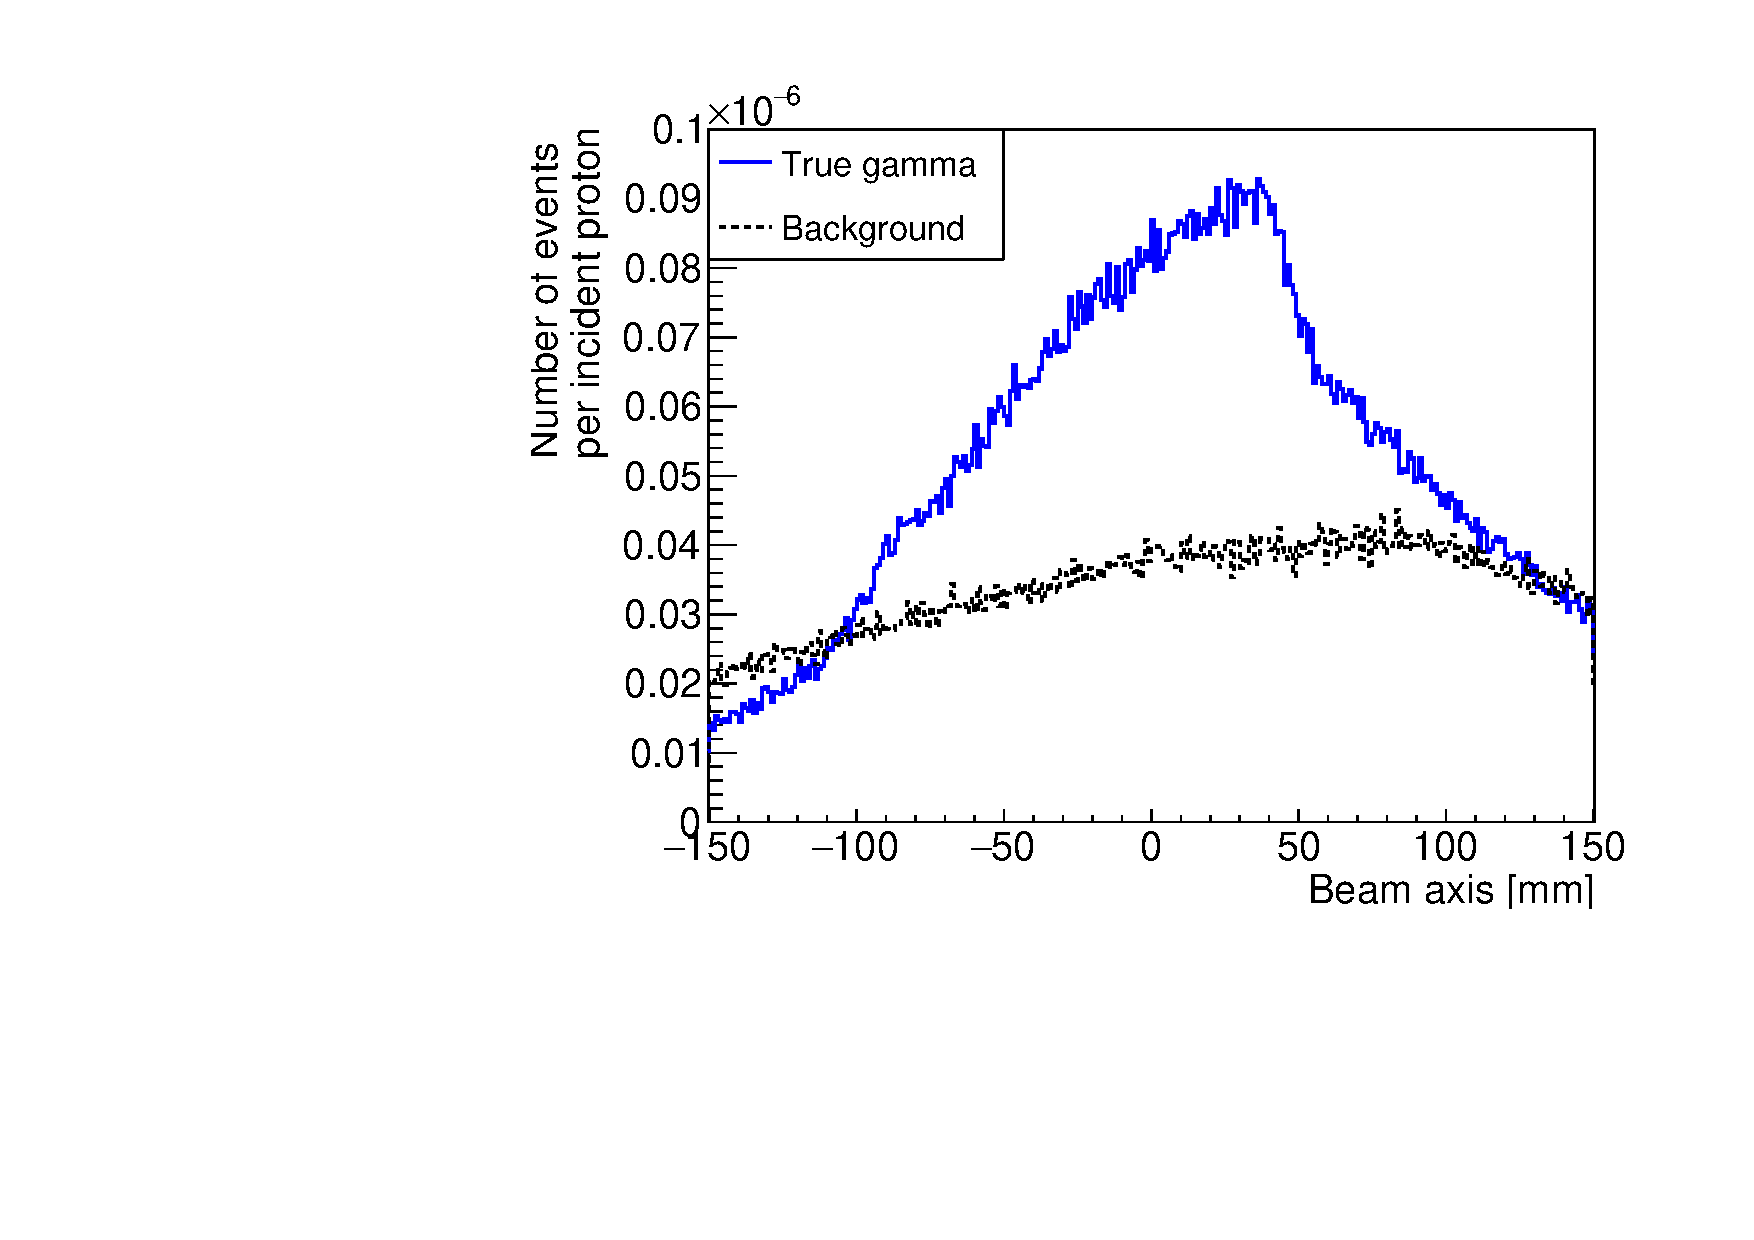
\includegraphics[width=0.33\textwidth]{./Figure/profile_high_stat_linecone_2.pdf}}
% \subfloat[\label{fig:fig_Results_Estimation_Camera_Profil_highStat_CC_simulation_Hadronth_MLEM}]{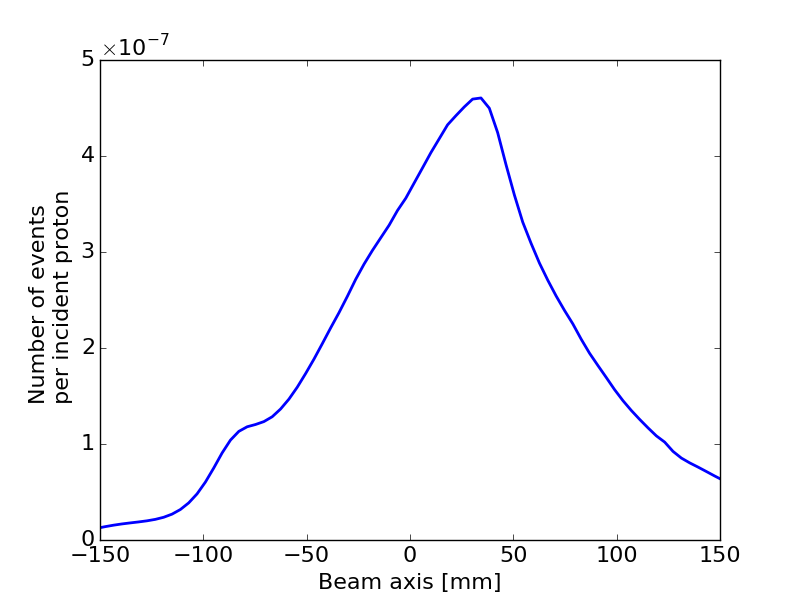
\includegraphics[width=0.32\textwidth]{./Figure/profileY_corr_r15.png}}\\
%  %\subfloat[\label{fig:fig_Estimation_Camera_CC_NURBS_Poisson_LC}]{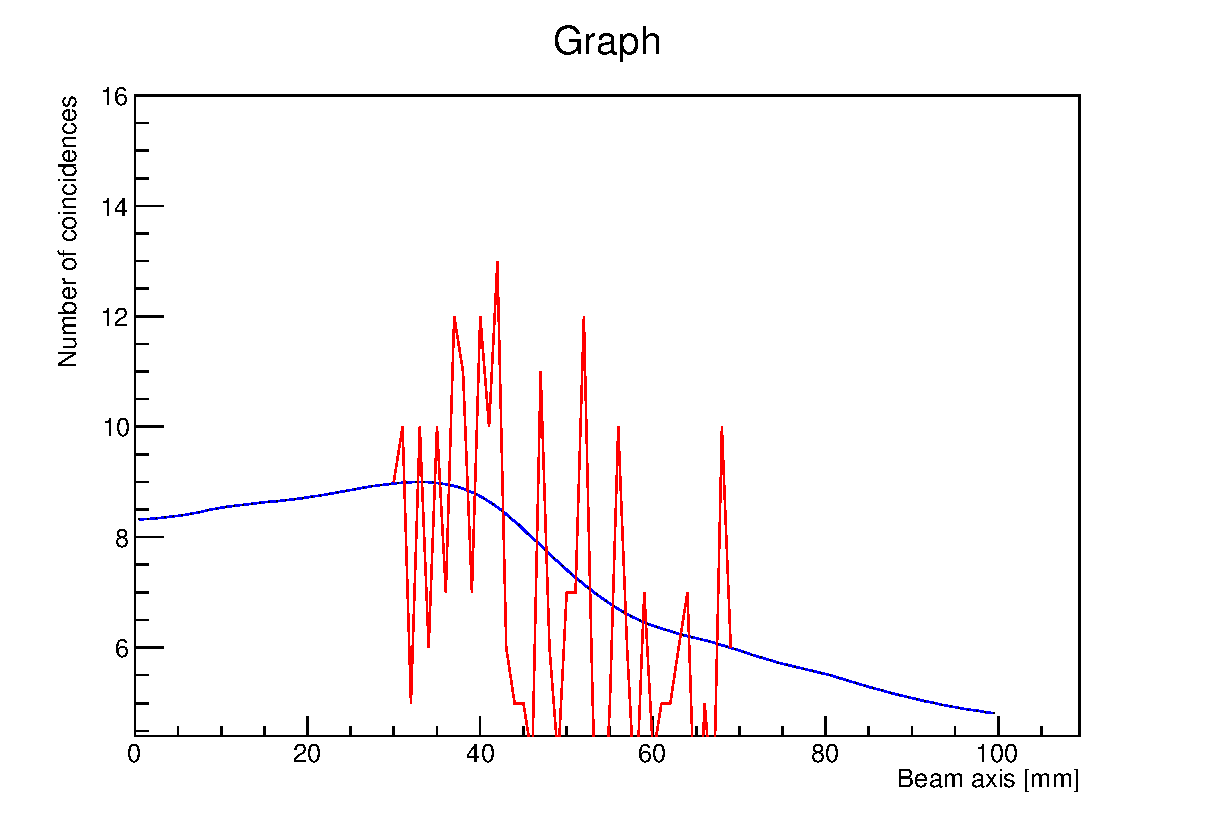
\includegraphics[width=0.33\textwidth]{./Figure/2017-08-02_Poisson_Nurbs_1e8_Article_LC.eps}}
%  \subfloat[\label{fig:fig_Estimation_Camera_CC_NURBS_Poisson_LC}]{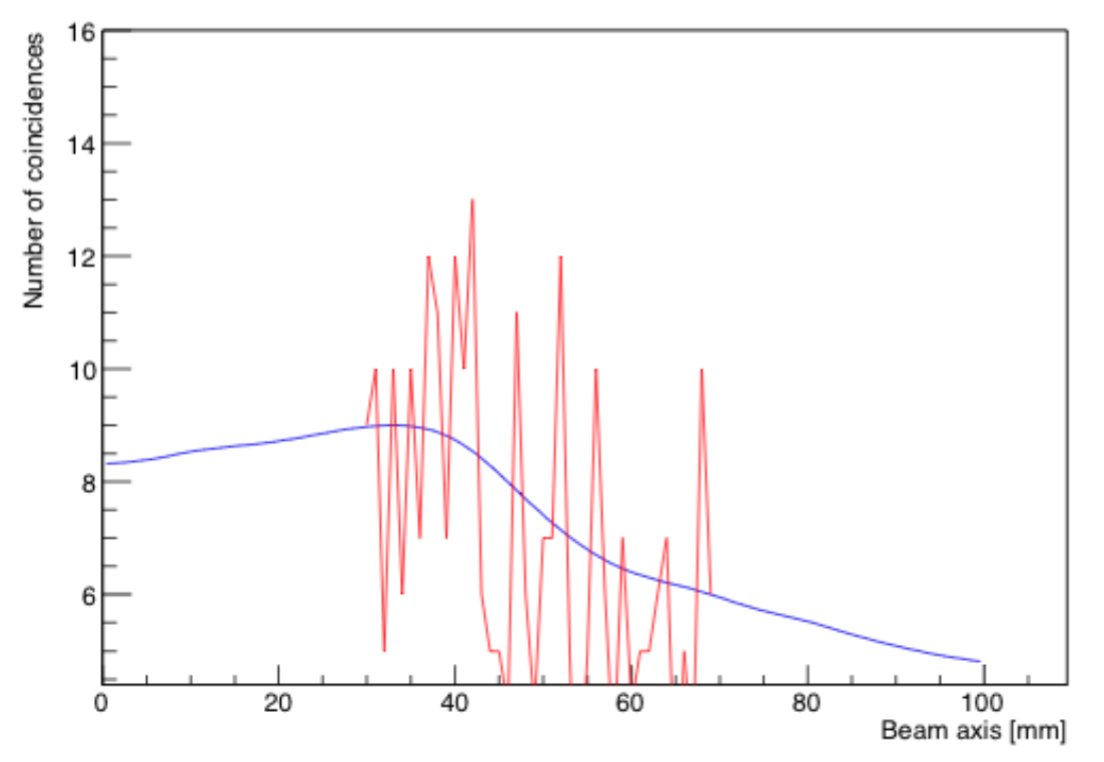
\includegraphics[width=0.33\textwidth]{./Figure/line_cone_NURBS.png}}
%  %\subfloat[\label{fig:fig_Estimation_Camera_CC_NURBS_Poisson_MLEM}]{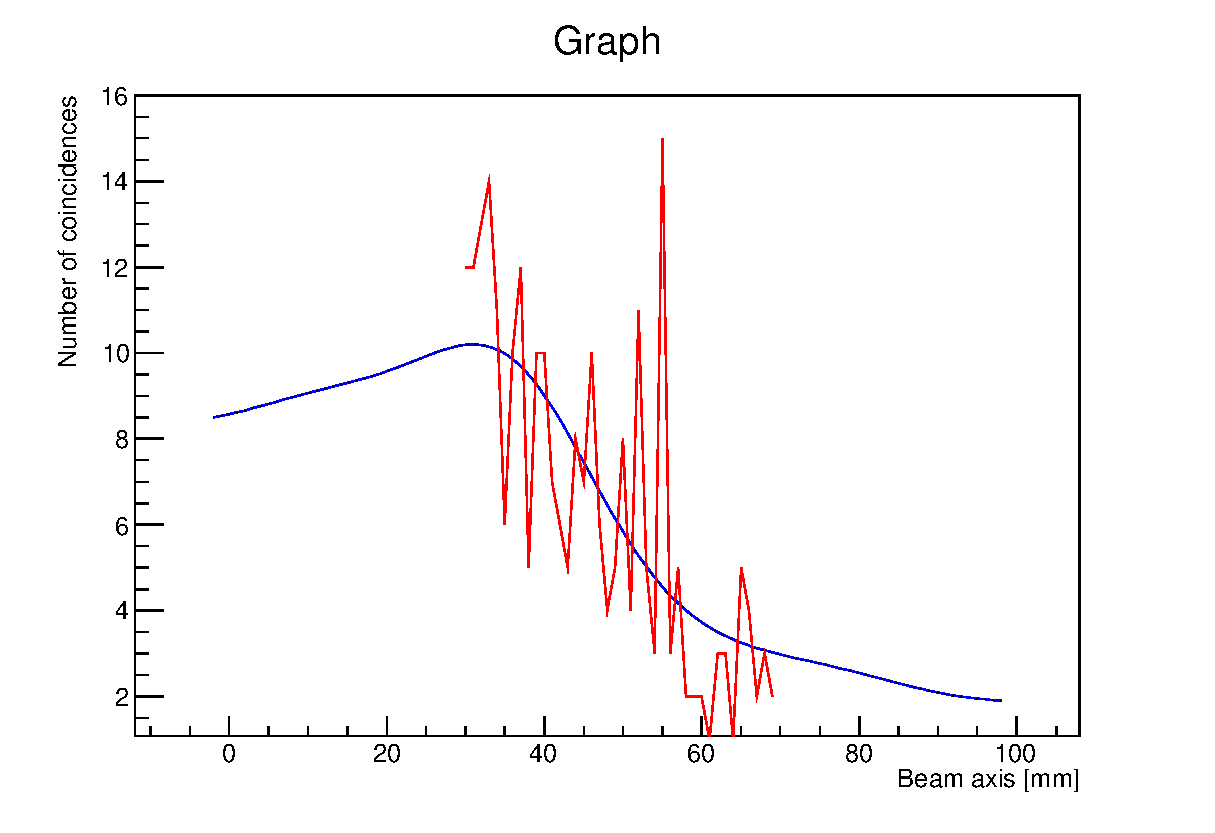
\includegraphics[width=0.33\textwidth]{./Figure/2017-08-02_Nurbs_Poisson_1e8_Article_MLEM.eps}}\\
%  \subfloat[\label{fig:fig_Estimation_Camera_CC_NURBS_Poisson_MLEM}]{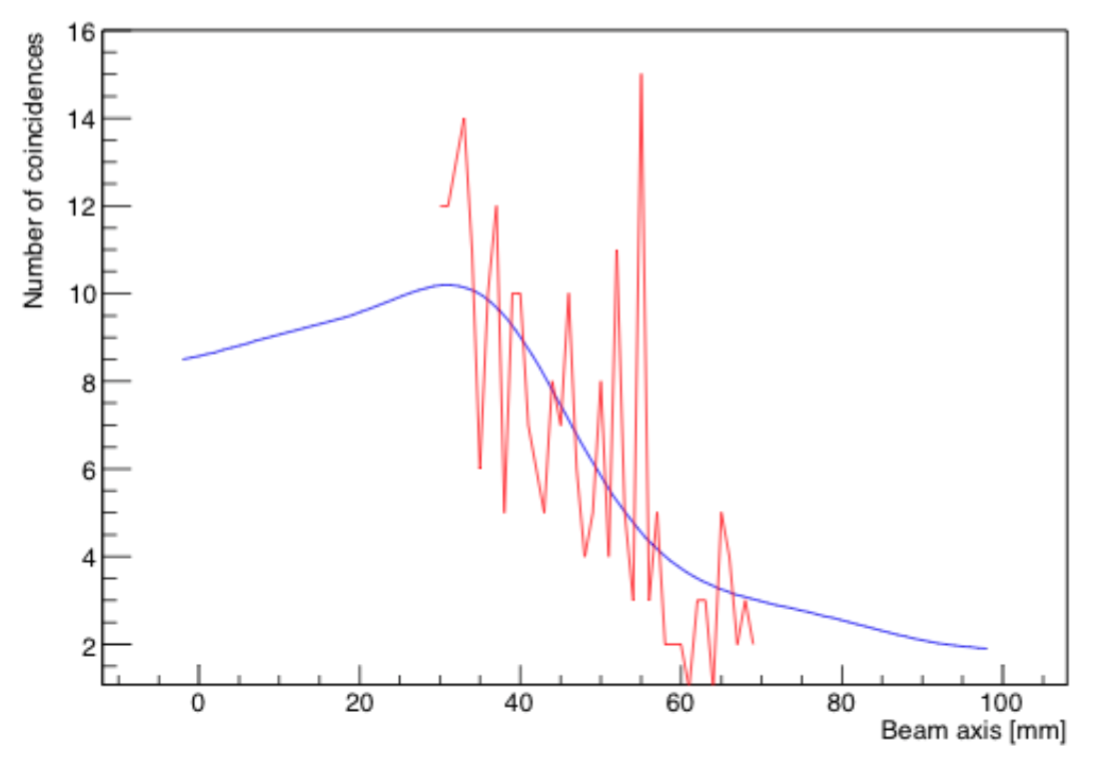
\includegraphics[width=0.33\textwidth]{./Figure/MLEM_NURBS.png}}\\
%   %\subfloat[\label{fig:fig_Results_Chi2_Distribution_Variation_CC_simulation_Hadronth_LC}]{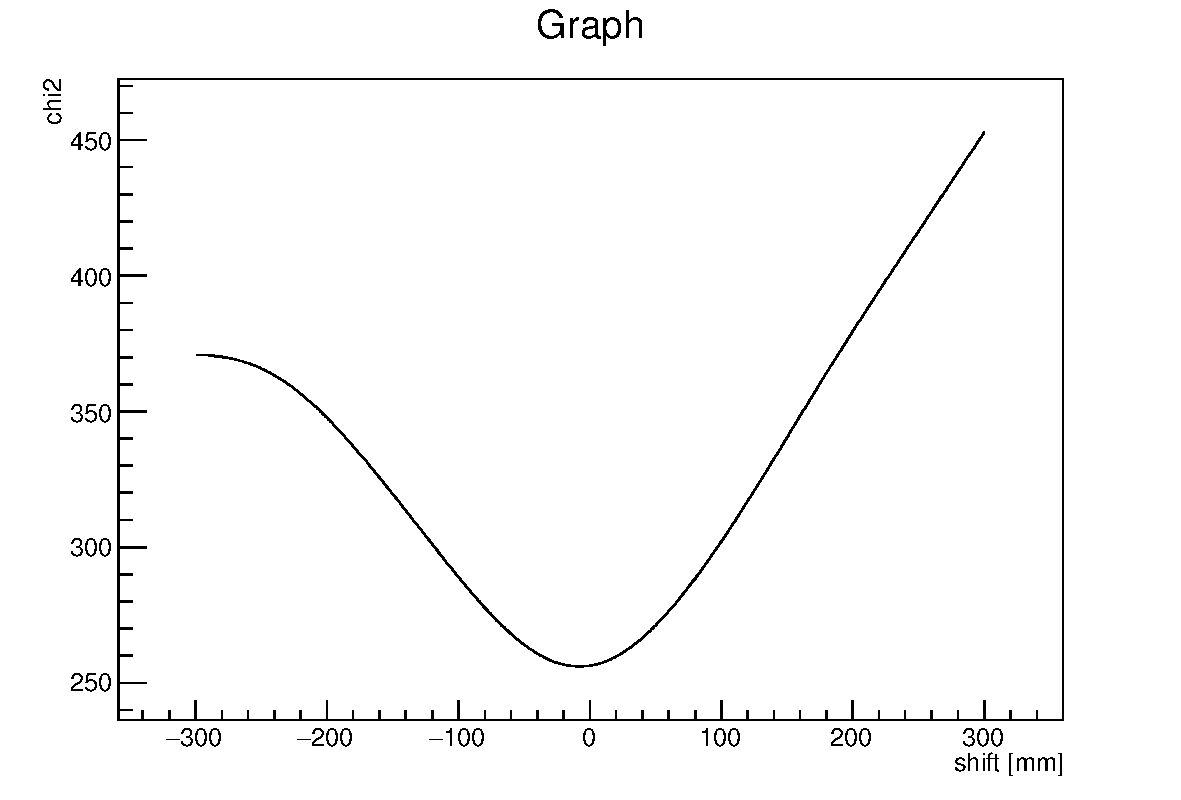
\includegraphics[width=0.33\textwidth]{./Figure/2017-08-02_Distribution_Chi2_1e8_LC.pdf}}
%   \subfloat[\label{fig:fig_Results_Chi2_Distribution_Variation_CC_simulation_Hadronth_LC}]{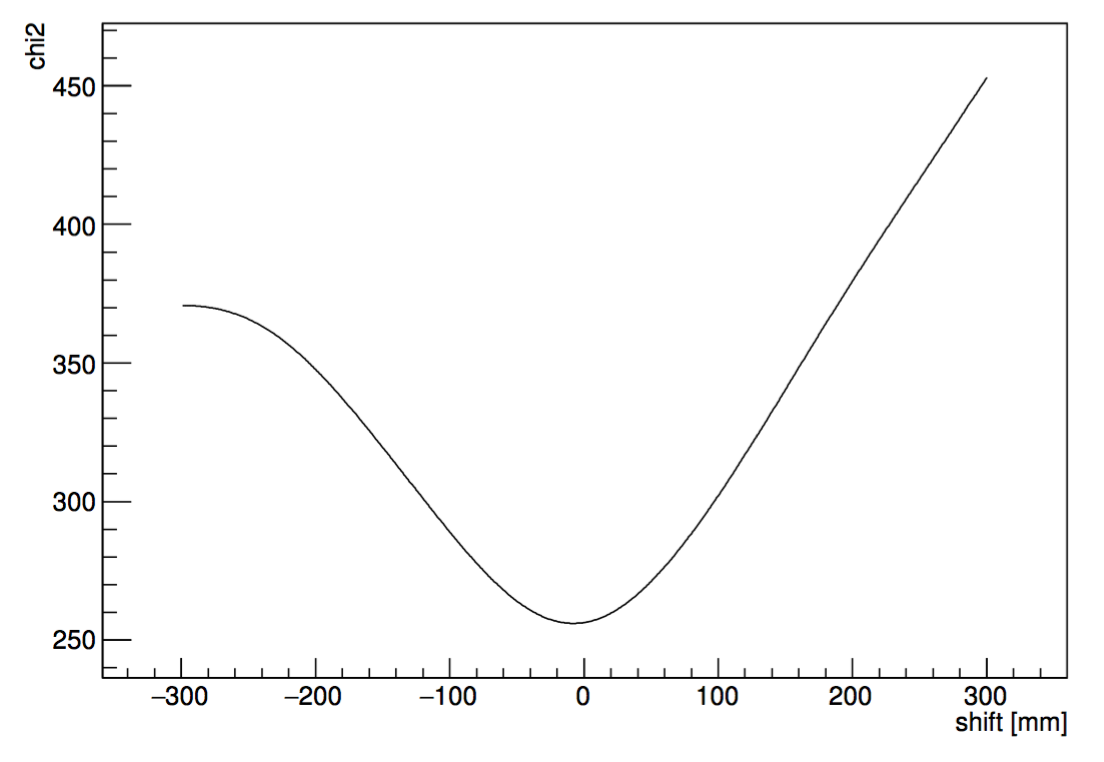
\includegraphics[width=0.33\textwidth]{./Figure/chi2_linecone.png}}
%  %\subfloat[\label{fig:fig_Results_Chi2_Distribution_Variation_CC_simulation_Hadronth_MLEM}]{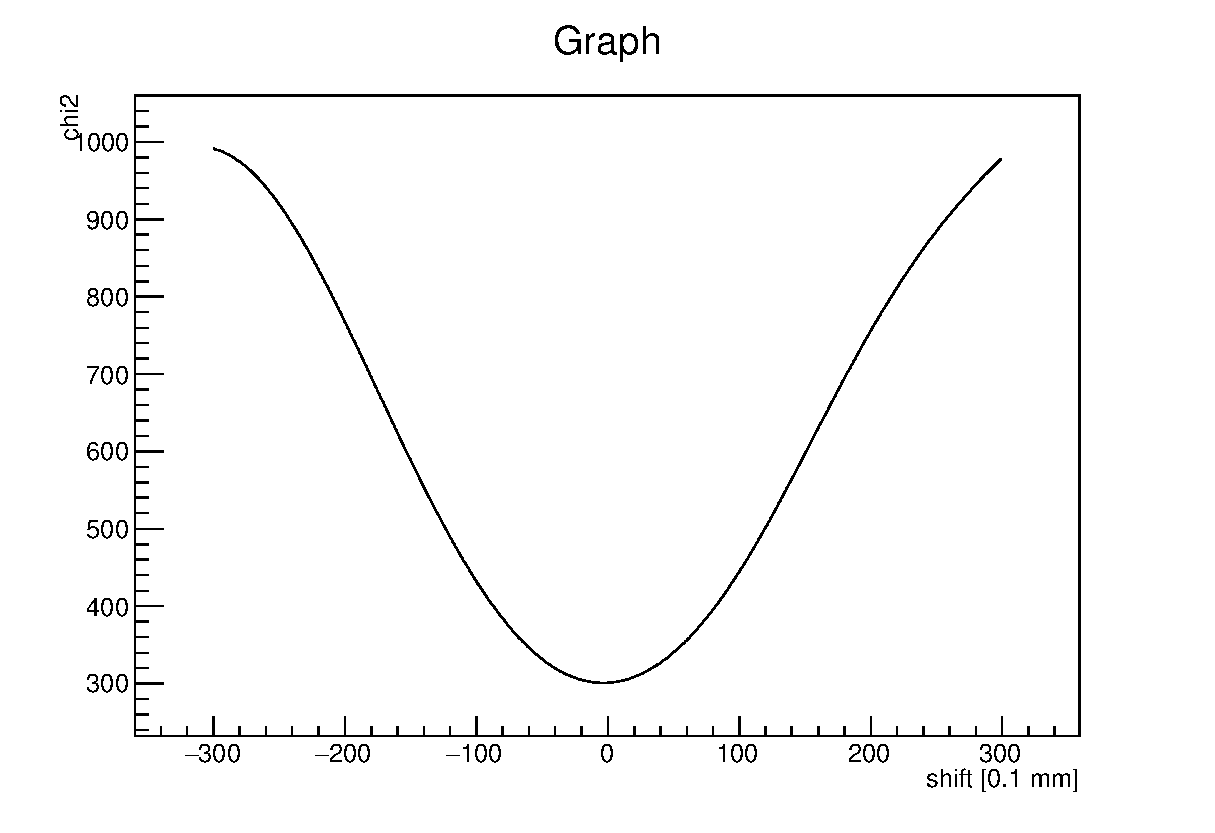
\includegraphics[width=0.33\textwidth]{./Figure/2017-08-02_Distribution_Chi2_Results_binning_1mm_ShiftNurbs0_1mm_1e8_article_MLEM.eps}}\\
%  \subfloat[\label{fig:fig_Results_Chi2_Distribution_Variation_CC_simulation_Hadronth_MLEM}]{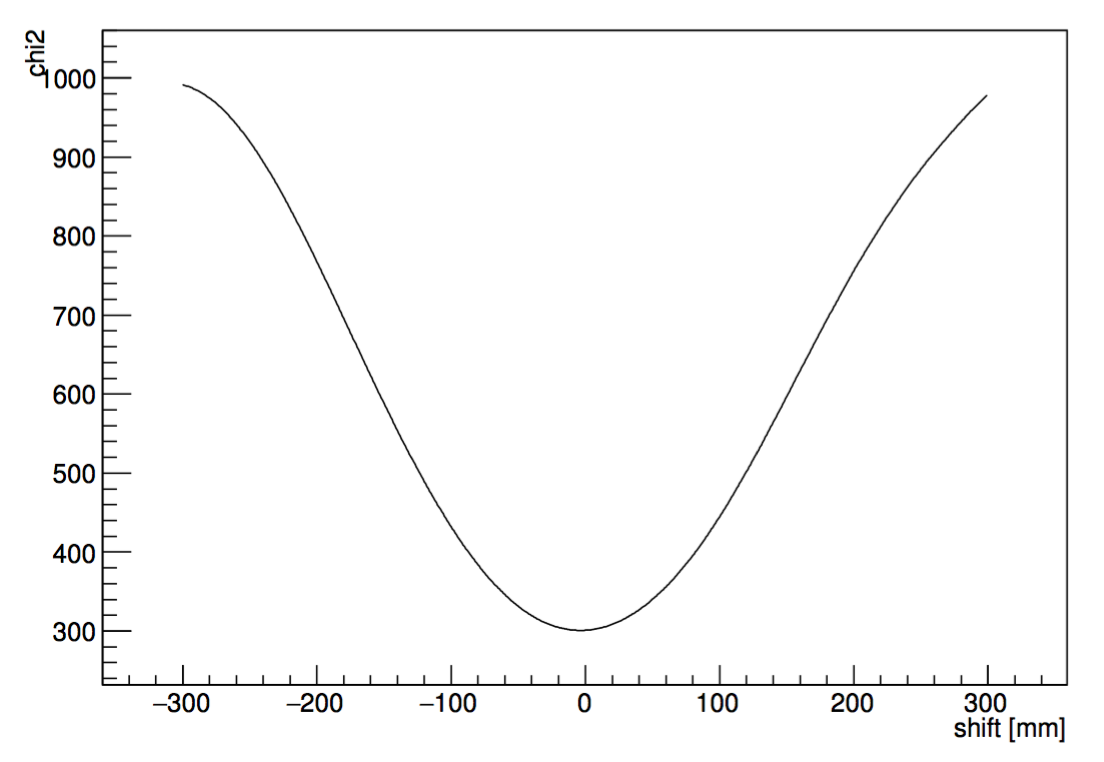
\includegraphics[width=0.33\textwidth]{./Figure/chi2_MLEM.png}}\\
%   %\subfloat[\label{fig:fig_Results_Precision_Distribution_Variation_CC_simulation_Hadronth_LC} ]{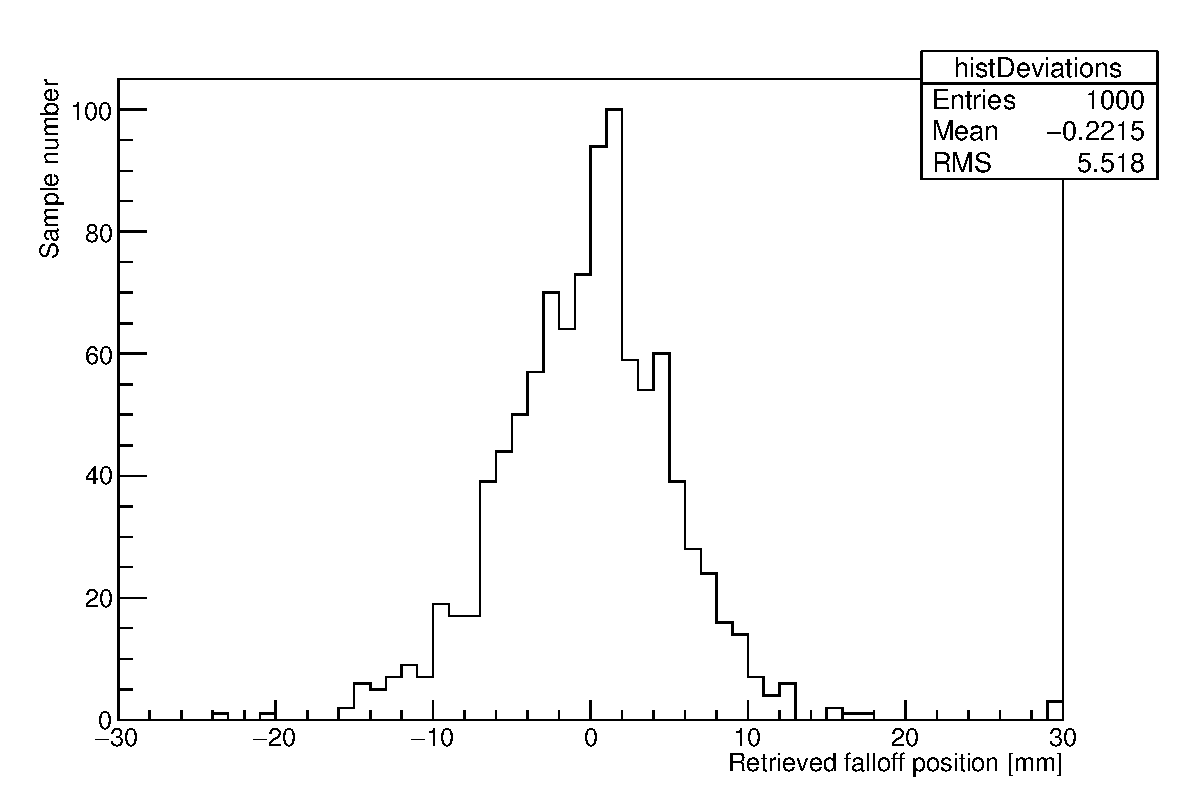
\includegraphics[width=0.33\textwidth]{./Figure/2017-08-02_Distribution_finale_1e8_Article_LC.pdf}}
%   \subfloat[\label{fig:fig_Results_Precision_Distribution_Variation_CC_simulation_Hadronth_LC} ]{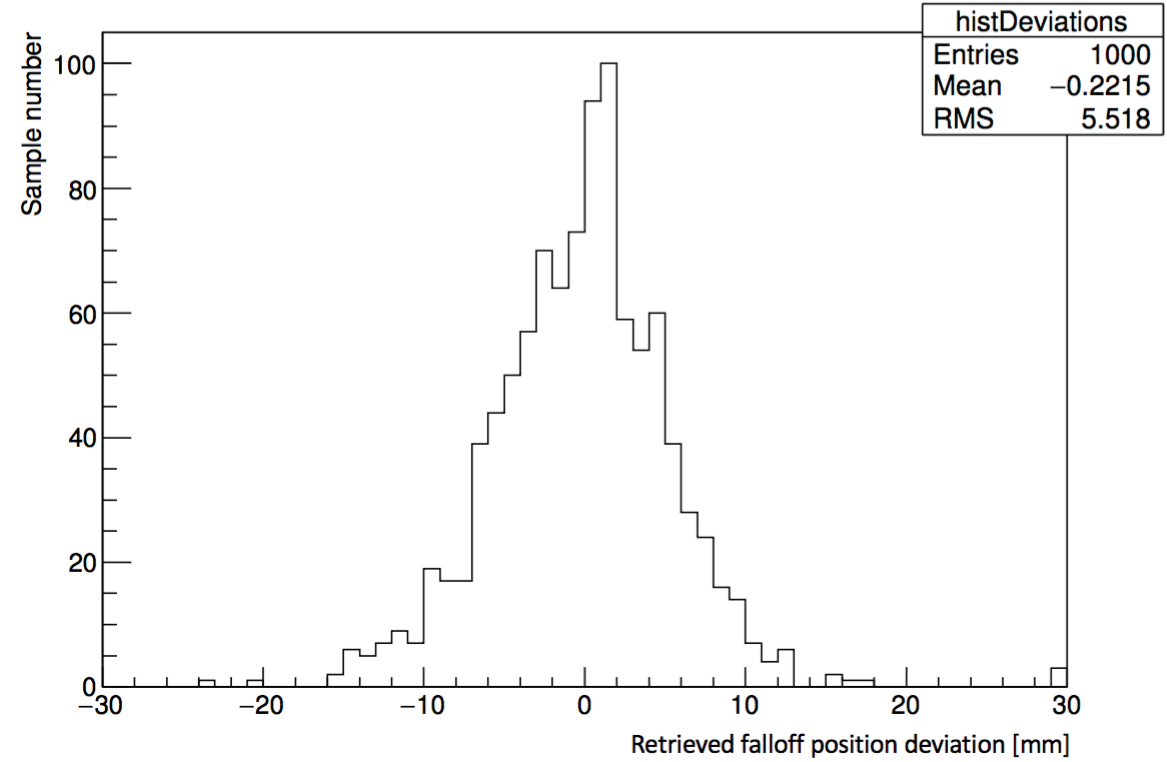
\includegraphics[width=0.33\textwidth]{./Figure/deviation_linecone.png}}
%  %\subfloat[\label{fig:fig_Results_Precision_Distribution_Variation_CC_simulation_Hadronth_MLEM} ]{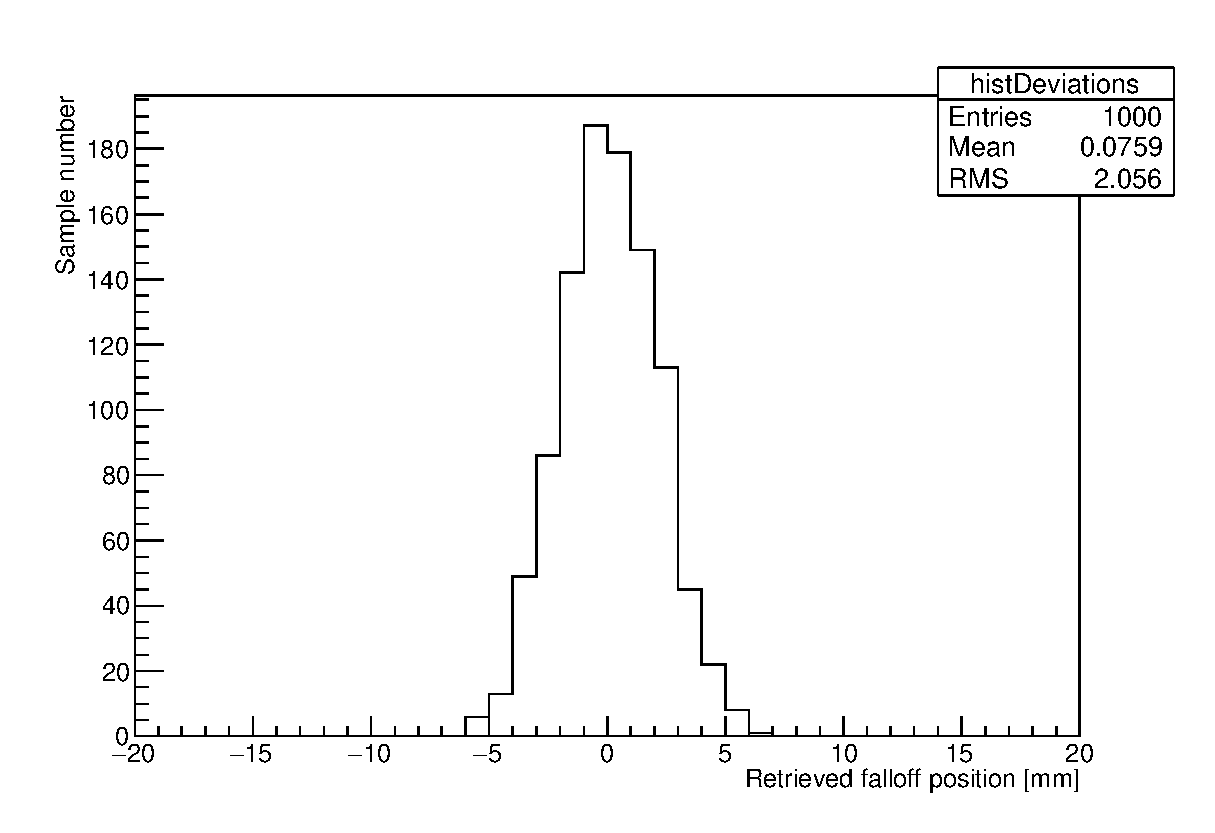
\includegraphics[width=0.33\textwidth]{./Figure/2017-08-02_FallOff_Results_binning_1mm_ShiftNurbs0_1mm_1e8_Article_MLEM.eps}}
%  \subfloat[\label{fig:fig_Results_Precision_Distribution_Variation_CC_simulation_Hadronth_MLEM} ]{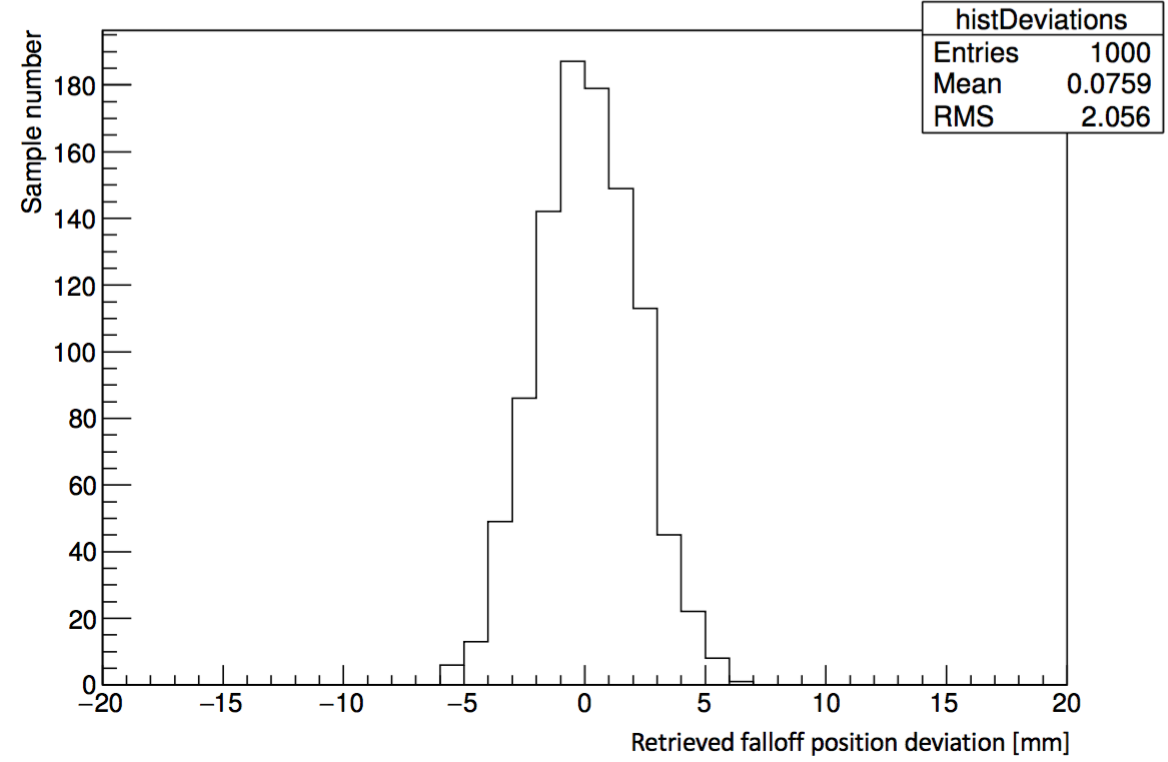
\includegraphics[width=0.33\textwidth]{./Figure/deviation_MLEM.png}}
% \caption{Data processing comparison for the same proton simulation with the line cone algorithm (left column) and the LM-MLEM algorithm (right column). The first row gives the reconstructed profile for $10^{10}$ incident protons. The second row shows the reference curve (blue) and the curve obtained with a $10^8$ incident protons subset. The third row shows the $\chi^2$ distribution for one data subset. The last row represents the distribution of the minimal calculated shifts for 1000 subsets at the same statistics of $10^8$ incident protons.}
% \end{figure}

